% !Mode:: "TeX:UTF-8"
%\documentclass[twocolumn]{sig-alternate}
\documentclass[10pt,conference,compsocconf,letterpaper]{IEEEtran}
%\documentclass[twocolumn,10pt]{infocom}
%\documentclass[twocolumn,10pt]{IEEEtran_v15}
%\documentclass[twocolumn,10pt]{IEEEtran}
%\documentclass[twocolumn,10pt]{article}
%\usepackage[sort,nocompress,space]{cite}
%\documentclass[letterpaper,twocolumn,10pt]{article}
%\usepackage{usenix,epsfig,endnotes}
%\usepackage[letterpaper]{geometry}

%\usepackage{ifpdf}
%\ifpdf
%\setlength{\pdfpagewidth}{8.5in}
%\setlength{\pdfpageheight}{11in}
%\else
%\fi

%%%%%%%%%%%%%%%%%%%%%%
% Set Compact Mode   %
%%%%%%%%%%%%%%%%%%%%%%

%\newcommand{\subparagraph}{}


%\usepackage[compact]{titlesec}
%\titlespacing{\section}{0pt}{*0}{*0}
%\titlespacing{\subsection}{0pt}{*0}{*0}
%\titlespacing{\subsubsection}{0pt}{*0}{*0}
%\setlength{\parskip}{0pt}
%\setlength{\parsep}{0pt}
%\setlength{\headsep}{0pt}
%\setlength{\topskip}{0pt}
%\setlength{\topmargin}{0pt}
%\setlength{\topsep}{0pt}
%\setlength{\partopsep}{0pt}
%\setlength{\itemsep}{0pt}

%%%%%%%%%%%%%%%%%%%%%%
%
%%%%%%%%%%%%%%%%%%%%%%


\usepackage{url}
\usepackage[sort,space]{cite}
\usepackage{lineno}
\renewcommand\linenumberfont{\normalfont\bfseries\small}
\usepackage{pifont}
\usepackage{epsfig,epsf,url,amssymb}
\usepackage{tabularx}
%\usepackage{algorithm2e}
\usepackage[ruled,vlined]{algorithm2e}
\usepackage{algpseudocode}
\usepackage{amsmath}
\usepackage{mathtools}
\newtheorem{mydef}{Definition}
\usepackage{rotating}
\usepackage{wrapfig}
\usepackage{times}
\long\def\comment#1{}
\usepackage{multirow}
\usepackage{lscape}
\usepackage{stmaryrd}
\usepackage{wrapfig}
\usepackage{hhline}
\usepackage{textcomp,booktabs}
\usepackage[usenames,dvipsnames]{color}
\usepackage{colortbl}
\usepackage{multirow}
\usepackage{rotating}
\usepackage{epstopdf}
\definecolor{mygray}{gray}{.9}
\definecolor{mypink}{gray}{.9}
\definecolor{mycyan}{cmyk}{.3,0,0,0}

\usepackage{graphicx}
%\usepackage{subfigure}
\usepackage{subfig}
\usepackage[font=bf]{caption}

\newcommand{\bbR}{\mathbb{R}}
\newcommand{\calN}{\mathcal{N}}
\newcommand{\calR}{\mathcal{R}}
\newcommand{\calV}{\mathcal{V}}
\newcommand{\eg}{{\it e.g.}}
\newcommand{\etal}{{\it et al.~}}
\newcommand{\etc}{{\it etc.}}
\newcommand{\ie}{{\it i.e.}}
\newcommand{\tablecapspace}{{\vspace{-0.1in}}}
\newcommand{\tablespace}{{\vspace{-0.05in}}}
\newcommand{\picspace}{{\vspace{-0.1in}}}
\renewcommand{\baselinestretch}{1}
\renewcommand{\arraystretch}{1.05}      % make the space between tabular lines larger
\newcommand{\capspace}{}           % control space between figure/table and caption

\def\TODO#1{\textcolor{red}{#1}}

%\setlength{\textheight}{9.3in}
%\setlength{\columnsep}{1.4pc}
%\setlength{\textwidth}{7.1in}

\newcommand{\sys}{{\textsf{Trinity}}\xspace}

\newcommand{\paragraphb}[1]{\vspace{0.05in}\noindent{\bf #1}}

\newcommand{\paraspace}{\vspace{0.03in}}
\newcommand{\parab}[1]{\paraspace\noindent{\bf #1} }
\newcommand{\parae}[1]{\paraspace\noindent{\em #1} }
\newcommand{\parabe}[1]{\paraspace\noindent{\bf \em #1} }
\newcommand{\kai}[1]{{\color{blue}[Kai: #1]}}
\newcommand{\chen}[1]{\color{green}[Chen: #1]}
\newcommand{\ying}[1]{{\color{red}[Ying: #1]}}
\newcommand{\shuihai}[1]{{\color{red}#1}}
\def\naive{na\"\i ve}

\newcommand{\tabincell}[2]{\begin{tabular}{@{}#1@{}}#2\end{tabular}}

\newcommand{\subcaption}[1]{\centerline{#1}\vspace{0.1in}}
\long\def\comment#1{}
\newtheorem{theorem}{Theorem}
\newtheorem{lemma}[theorem]{Lemma}
\newtheorem{proposition}[theorem]{Proposition}
\newtheorem{corollary}[theorem]{Corollary}
%\newtheorem{problem}[theorem]{Problem}

\newenvironment{definition}[1][Definition]{\begin{trivlist}
\item[\hskip \labelsep {\bfseries #1}]}{\end{trivlist}}
\newenvironment{problem}[1][]{\begin{trivlist}
\item[\hskip \labelsep {\bfseries}]}{\end{trivlist}}
\newenvironment{remark}[1][Remark]{\begin{trivlist}
\item[\hskip \labelsep {\bfseries #1}]}{\end{trivlist}}

\newenvironment{icompact}{
  \begin{list}{$\bullet$}{
    \parsep 1pt plus 1pt
    \partopsep 1pt plus 1pt
    \topsep 1pt plus 2pt minus 1pt
    \itemsep 1.5pt plus 1pt
    \parskip 0pt plus 2pt
    \leftmargin 0.15in}
       }
  {\normalsize\end{list}}

\newenvironment{ecompact}{
  \begin{list}{$\bullet$}{
    \parsep 1pt plus 1pt
    \partopsep 1pt plus 1pt
    \topsep 1pt plus 2pt minus 1pt
    \itemsep 1.5pt plus 1pt
    \parskip 0pt plus 2pt
    \leftmargin 0.15in}
       }
  {\normalsize\end{list}}


%%%%%%%% to calculate the time %%%%%%%%%%%%%%%%%%%%%%%%%%%%
\newcount\hour \newcount\minute
\hour=\time  \divide \hour by 60
\minute=\time
\loop \ifnum \minute > 59 \advance \minute by -60 \repeat
\def\drafttime{\ifnum \hour<13 \number\hour:%
                      \ifnum \minute<10 0\fi
                      \number\minute
                      \ifnum \hour<12 \ AM\else \ PM\fi
         \else \advance \hour by -12 \number\hour:%
                      \ifnum \minute<10 0\fi
                      \number\minute \ PM\fi}
\def\timestamp{\today \ \drafttime}

\begin{document}
%%\conferenceinfo{SIGCOMM,} {XXXXXX, XXXXX, XXXXX, XXXXX.} %
%%\CopyrightYear{2009} \crdata{1-59593-308-5/06/0009}
%
%%\title{SmartMarker: Isolating Network Performance \\ with Priority Coloring}
\title{Modelling deadlock with graph theory}
%\author{
%Shuihai Hu$^{1}$, Wei Bai$^{1}$, Kai Chen$^{1}$, Chen Tian$^{2}$, Ying Zhang$^{3}$, Haitao Wu$^{4}$\\
%$^{1}$SING Group @ HKUST~~~$^{2}$Nanjing University~~~$^{3}$HP Labs~~~$^{4}$Microsoft}
%
%%\author{Paper $\# 851$, $9$ pages}
\maketitle
%
%\begin{abstract} Remote Direct Memory Access over Converged Ethernet (RoCE) deployments
		are vulnerable to deadlocks induced by Priority Flow Control (PFC).
		Prior solutions for deadlock prevention either require significant
		changes to routing protocols, or require excessive buffers in the
		switches. In this paper, we propose a scheme for deadlock prevention,
		called \sysname{}. It does not require any changes to the routing
		protocol, and needs only modest buffers.  \sysname{} is based on the
		insight that given a set of expected lossless routes, a simple tagging
		scheme can be developed to ensure that no deadlock will occur under any
		failure conditions. We design such a scheme, prove that it prevents
		deadlock and implement it efficiently on commodity hardware.
\end{abstract}

%\vspace{-0.1in}
\section{Introduction}\label{sec:intro}

Driven by the need for ultra-low latency, high throughput and low CPU overhead, both Microsoft and Google are deploying Remote Direct Memory Access (RDMA) in their datacenter networks in recent years~\cite{dcqcn,timely}. Among the available RDMA technologies,  RDMA over Converged Ethernet (RoCE)~\cite{roce} is a promising one as it is compatible with current IP and Ethernet based datacenter networks.

The deployment of RoCE requires Priority-based Flow Control (PFC)~\cite{pfc} to provide a lossless L2 network. With PFC, packet loss can be avoided by letting a switch pause its immediate upstream device before buffer overflow occurs. However, the adoption of PFC will cause deadlock problem. Deadlock refers to such a standstill situation: There is a cyclic buffer dependency among a set of switches. Any switch in the cycle holds all the buffer needed by its upstream switch, and meanwhile is waiting for its downstream switch to release some buffer and resume its packet transmission.

It is easy to see that when deadlock occurs, no switch in the cycle can proceed. Further, throughput of the whole network or part of the network will go to zero due to the backpressure effect of PFC pause. Hence it is necessary to design some mechanisms for handling deadlock problem when deploying RDMA in datacenter networks. 

Prior works on preventing deadlock can be roughly classified into two categories including 1) \textit{Routing restriction based approach}~\cite{tcpbolt,flich2012survey}. The idea of this approach is to ensure that no cyclic buffer dependency exists in the network by limiting the routing paths used in each priority class;  2) \textit{buffer management (structured buffer pool) based approach}~\cite{gerla1980flow,karol2003prevention}. This approach divides switch buffer into several buffer classes. A packet is allowed to access more buffer classes as it travels greater distance in the network. It can be proved that as long as the number of buffer classes is no smaller than the hop count of the longest routing path, there will be no cyclic buffer dependency in the network.


These two kinds of approaches are known to have some important drawbacks. For example, routing restriction based approach usually wastes link bandwidth and limits throughput performance, while buffer management based approach introduces non-trivial deployment complexity to the network system. The drawbacks of these approaches somehow can be viewed as the cost to eliminate cyclic buffer dependency in the network, which has been identified as the primary principle for designing a deadlock prevention solution.

Though obeying this principle can guarantee a deadlock-free network, its cost can be very expensive. In this paper, instead of seeking a solution that introduces less overhead, we take one step back and ask: Is cyclic buffer dependency a sufficient and necessary condition for deadlock? Or can deadlock-free be guaranteed without eliminating cyclic buffer dependency?

To answer the above questions, we did some study about several representative deadlock cases. Our findings are as follows. First, cyclic buffer dependency is just a necessary condition for deadlock. There are some cases where cyclic buffer dependency is met, but there is no deadlock. Second, even if all the links in a switch cycle are paused simultaneously, deadlock may still not occur. These two findings indicate that prior solutions are designed based on a too strict condition, and thus introduces some unnecessary overhead. 
\todo{(We need a much better discussion here, let's discuss how to argue that our deadlock case study is important and meaningful.)}


%1)\textit{Routing restriction based approach}. The idea is to limit the routing paths used in a network to ensure that there is no cyclic buffer dependency; 2)\textit{Priority class based approach.} This approach splits each physical link into several priority classes, and associates each class with some dedicated buffer at each hop. Within each priority class, only deadlock-free routes are allowed to be installed, so there will be no deadlock. 3)\textit{buffer management (structured buffer pool) based approach}. This approach divides switch buffer into several buffer classes. A packet is allowed to access more buffer classes as it travels greater distance in the network. It has been proved that as long as the number of buffer classes is no smaller than the hop count of the longest routing path in the network, there will be no deadlock. 
%\section{Background}
\label{sec:background}

We now provide a brief primer on RDMA, RoCE, the problem of deadlocks and prior
work in this area.

{\bf RDMA and RoCE:} Remote Direct Memory Access (RDMA) technology offers high
throughput, low latency and low CPU overhead, by bypassing end-host networking
stacks. Instead, Network Interface Cards(NICS) transfer data in and out of
pre-registered memory buffers at the two end hosts.  In modern data centers,
RDMA is deployed using RDMA over Converged Ethernet V2 (RoCE)
standard~\cite{roce,rroce}

{\bf PFC:} RoCE needs a lossless L2 layer for optimal performance. This is
accomplished in Ethernet networks using the Priority Flow Control (PFC)
mechanism~\cite{pfc}.  Using PFC, a switch can pause an incoming link when its
ingress buffer occupancy reaches a preset threshold. As long as sufficient
``headroom'' is reserved to buffer packets that are in flight during the time
takes for the PAUSE to take effect, no packet will be dropped due to buffer
overflow~\cite{cisco-whitepaper,dcqcn}. 

The PFC standard defines 8 classes\footnote{Although, only one or two can be
used in practice -- see \S\ref{subsec:pfcheadroom}.}, called priorities~\footnote{The word priority is a
misnomer. There is no implicit ordering among priorities -- they are really just
separate classes.}. Packets in each priority are buffered separately, and PAUSE
messages carry this priority.  When a packet arrives at port $i$ of switch $S$
with priority $j$, it is enqueued in queue $j$ of port $i$. If the queue length
now exceeds the PFC threshold, a pause message (XOFF) is sent to the upstream
switch connected to port $i$. The message carries priority $j$. The upstream
switch then stops sending packets with priority $j$ to switch $S$ on port $i$ until a resume
message (XOFF) with priority $j$ is received.

PFC prevents buffer overflow, but it can lead to deadlocks.

%% Since PAUsing is carried out
%% on a per-ingress port, and not on a per-flow basis, problems such as unfairness
%% and head-of-the-line blocking may occur~\cite{dcqcn}. The PFC standard defines 8
%% classes (called priorities), where packets in class are buffered separately, to
%% mitigate these problems~\cite{dcqcn}. However, sine each priority needs its own
%% dedicated headroom, typically, no more than two or three priorities are
%% used~\cite{rdmaatscale}.

{\bf Deadlock:} Deadlock forms when paused links form a cycle
(Figure~\ref{fig:deadlock_example}). Once formed,
deadlock is ``permanent'' in the sense that it will continue to exist even if no
new traffic is injected into the loop. Deadlocks in PFC-based networks (or more
generally, in credit-flow networks) are a well-known problem. It is not merely a
theoretical problem -- it has been reported in practice~\cite{rdmaatscale}.

It is well known that Circular Buffer Dependency (CBD) is a {\em necessary}
condition for deadlock formation~\cite{tcp-bolt,hu2016deadlocks}. {\em
Sufficient} condition for deadlock formation in PFC networks have yet to be
fully understood~\cite{hu2016deadlocks}. 

{\bf Prior work on deadlock avoidance:} Prior work on deadlock management falls
in two categories: deadlock avoidance, or deadlock detection and resolution. Our
focus in this paper is on deadlock avoidance.  Since {\em sufficient} conditions
for deadlock formation are not well characterized, deadlock avoidance schemes
focus on preventing CBD for occurring. This is done either by limiting or
modifying routing~\cite{tcpbolt} to avoid CBD, or by careful buffer
management~\cite{xxx}. 

However, these schemes fail to meet one or more of the three key challenges:
$(i)$ they cannot be deployed with existing routing, or, $(ii)$ they do not deal
with dynamic nature of data center networks, or, $(iii)$ they require excessive
switch buffers or number of priorities. 

We now describe these three challenges in more detail. See \S\ref{sec:related}
for a detailed review of prior work.

%% Prior work on deadlock formation fails to meet the three challanges: first, they
%% do not work with To avoid such deadlocks, {\em deadlock-free
%% routing}~\cite{tcpbolt} has been proposed. It guarantees that (if the routing
%% configuration is correct,) any traffic does not cause deadlock.
%% 
%% Unfortunately, achieving deadlock-free routing is inefficient, and may not even
%% be viable. Deadlock-free routing is achieved by eliminating Cyclic Buffer
%% Dependency (CBD)~\cite{deadlockfree}.  However, ensuring that there is never any
%% CBD is challenging.
%% 
%% First, deadlock-free routing largely limits the choice of topology. For example,
%% Stephens et al. \cite{tcpbolt} proposes to only use tree-based topology and
%% routing, and shows that it is deadlock-free.  However, there are a number of
%% other datacenter topologies and routing schemes that are not
%% tree-based~\cite{bcube, camcube, jellyfish}, and do not have deadlock-free
%% guarantee.
%% 
%% Second, due to bugs or misconfiguration, deadlock-free routing configuration may
%% turn into deadlock-vulnerable. In fact, recent work has observed a PFC deadlock
%% case in real-world tree-based datacenter\cite{rdmascale}, caused by the
%% (unexpected) flooding of lossless class traffic.  Furthermore, there are
%% multiple reports of routing loops due to misconfiguration in today's production
%% datacenters~\cite{everflow, libra}. If lossless traffic encounters any of these
%% loops, CBD is unavoidable.  
%% 
%% Indeed, a recent paper~\cite{hu2016deadlocks} argued that preventing CBD is
%% quite difficult, so instead we should focus on defining and preventing
%% ``simpler''{\em sufficient} conditions to avoid deadlock. 
%% 
%% In this paper, we show that it is indeed possible to prevent CBD, in any
%% topology, without any changes to the underlying routing protocol, using existing
%% data center hardware. 





%\input{sections/sysoverview.tex}
%%\input{sections/overview.tex}
%%%\vspace{-0.1in}
\section{Solution}\label{sec:solution}
\todo{to be added.}
%\section{Implementation}\label{sec:implementation}

\sysname{} can be implemented by basic match-action functionality
available on most modern commodity switches. However, correct implementation
requires a key insight into the way PFC PAUSE frames are handled.

\begin{figure}
%	\hspace{-0.2in}
	\centering
	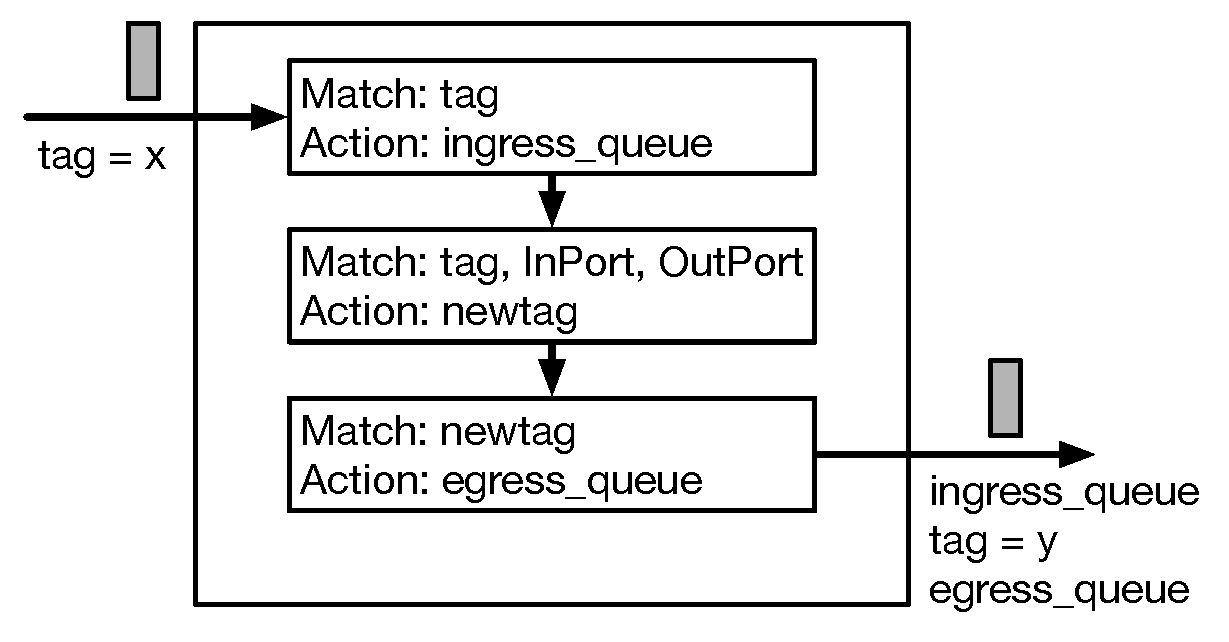
\includegraphics[width=0.42\textwidth] {figs/Tagger}
	%\vspace{-1em}
	\caption{Tagger match-action rules}\label{fig:tagger}
%	\vspace{-2em}
\end{figure}

\para {Match-Action rules:} \sysname{} needs to perform two operations at every
hop, i.e., {\em tag-based priority queueing} and {\em tag
rewriting}.  These two operations are implemented using a 3-step match-action
pipeline (Figure~\ref{fig:tagger}).  First, \sysname{} matches
the value of tags and classifies packets into ingress queues based. Second, 
\sysname{} matches (tag, InPort, OutPort) and rewrites the value of tag. 
The {\em third} step, wherein the packet is placed in an egress queue based on the
{\em new} tag value, is needed to ensure correct PFC operation, as described below.

\begin{figure}[t]
  %\vspace{-3em}
 	\centering
 	\subfloat[short for lof][Ingress priority = egress priority  $\rightarrow$ packet drop.] {
 	%	\vspace{-3em}
 		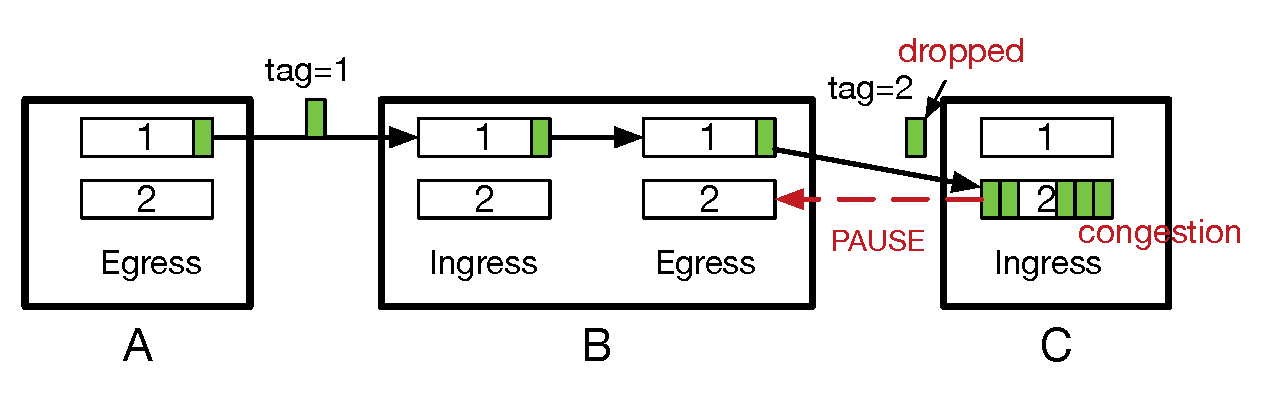
\includegraphics[width=0.42\textwidth] {figs/prioritydecoupling_1}
 	}
%  \vspace{-1.2em}
  
 	\subfloat[short for lof][Ingress priority = 1, egress priority = 2 $\rightarrow$ no drop.]{
 		%\vspace{-3em}
 		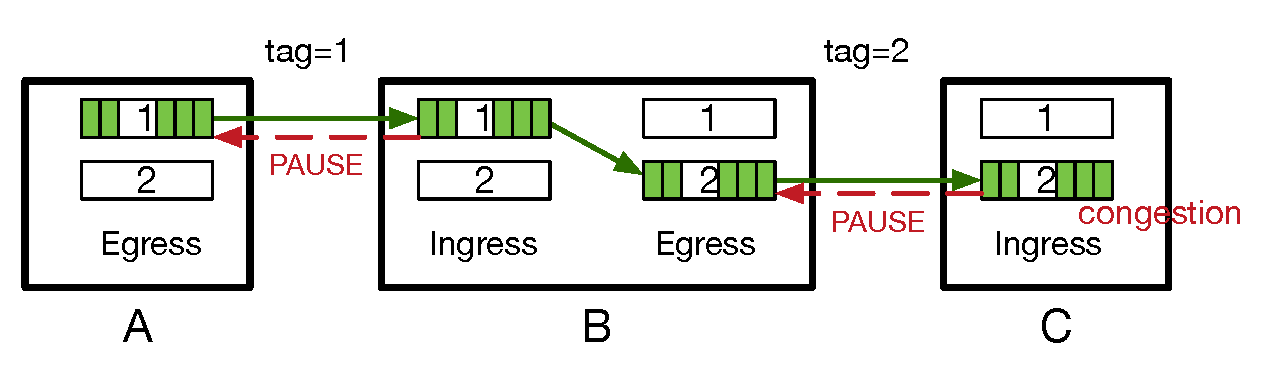
\includegraphics[width=0.42\textwidth] {figs/prioritydecoupling_2}
 	}
	 %\vspace{-1em}
 	\caption{Decoupling ingress priority from egress priority at switch B is necessary for lossless priority transition.}\label{fig:prioritydecoupling}
%	\vspace{-1em}
\end{figure}

\para{Handling priority transition:}
By default, a switch will enqueue a departing packet in the egress queue
of the same priority class as its ingress queue, as shown in Figure~\ref{fig:prioritydecoupling}(a).
In this example, Switch B is configured to 
perform priority transition for packets received from switch A and destined for switch C.
Packets exit egress queue 1 at switch B, but with priority 2. 
When ingress queue 2 of switch C becomes congested, the PFC PAUSE from switch C 
to switch B carries priority 2, and cannot pause the egress queue 1 of switch B.
This default behavior can lead to packet loss.

Therefore, we must map the packet to the egress queue
based on its new priority (Figure~\ref{fig:prioritydecoupling}(b)).  
This avoids packet loss, since the PFC from switch C
correctly pauses the queue on which the packet with the new tag would be
exiting.

\para{Rule compression:}  The match-action rules of \sysname{}
are implemented with TCAM. TCAM entries consist of {\em Pattern},
{\em Mask}, and {\em Result}. They refer to the pattern to be matched, the mask bits 
associated with the pattern and the action that occurs when a lookup hits the pattern, 
respectively.  One TCAM entry can have several Pattern-Mask pairs to match multiple packet header fields
simultaneously, e.g., an entry like (Pattern-1, Mask-1, Pattern-2, Mask-2, Result)
matches two fields simultaneously and fires only if both matches succeed.

\begin{figure}
	 
	\centering
	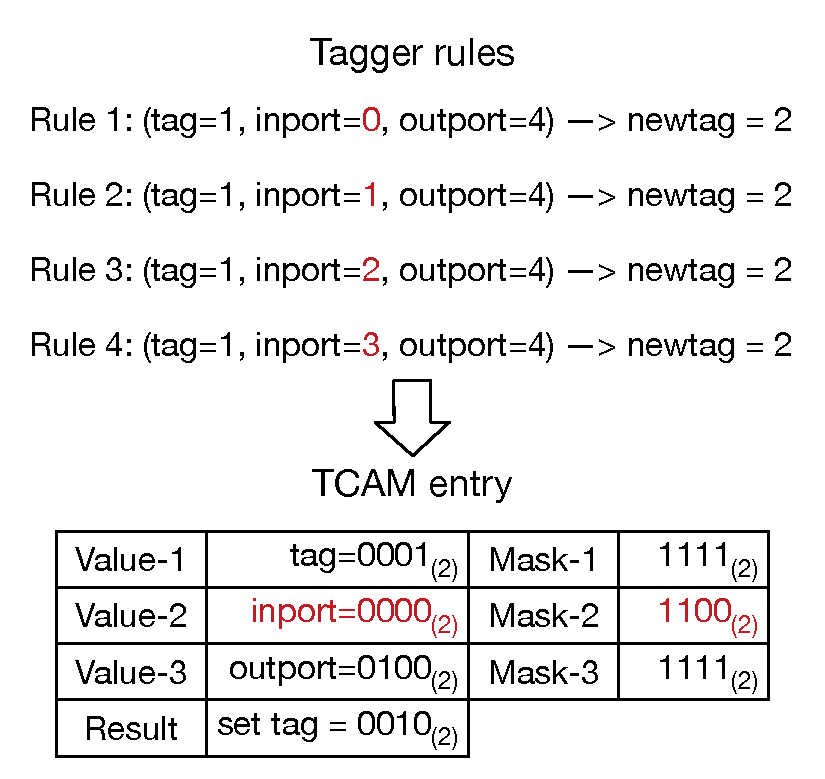
\includegraphics[width=0.37\textwidth] {figs/compression_with_bitmasking}
	\vspace{-1em}
	\caption{Rule compression with bit masking. Port numbers are bitmaps.
	The first bit from right represents port 0. The second bit represents port 1, and so on. }\label{fig:compression}
    \vspace{-1.5em}	
\end{figure}

Rules with the same Result can be compressed into one TCAM entry, if their
Patterns can be aggregated using bit masking. Consider the three
rules in Figure~\ref{fig:compression}. These rules are identical except the InPort
field in Pattern.

On commodity ASICs, port numbers in TCAM are bitmaps, not binary values. To match a single 
port, we can simply set the corresponding bit in the pattern to 1, and set the mask to all 1's. 
However, we may match multiple ports with one rule. We set the pattern to 
all 0's, and set the corresponding bits in the mask to 0. As shown in Figure~\ref{fig:compression},  
to match InPorts 0, 1 and 3, we set Pattern-2 to ``0000''  and Mask-2 to ``0100''. In this case, 
only the packet received from InPorts 0, 1 or 3 will match Pattern-2 after doing bit masking with Mask-2. 
Thus, the three rules are compressed into a single TCAM entry.

Recall from \S\ref{sec:generic} that without any compression, we need
$n(n-1)m(m-1)/2$ rules per switch. The number of rules can be
compressed to $nm(m-1)/2$ by aggregating InPorts.  The
result can be further improved by doing joint aggregation on tag, InPort and
OutPort.

\para{Broadcom implementation:} We implemented \sysname{} on commodity
switches based on Broadcom ASICs.  We use DSCP field in IP header as the tag.
The DSCP-based ingress priority queuing (step 1), ingress ACL and DSCP rewriting (step 2),
and ACL-based egress priority queuing (step 3) are well supported by the
commodity ASICs and do not require any ASIC changes. \shuihai{Everything is implemented using available and documented functionality.}

%Everything is implemented using publicly available and documented functionality.

%DSCP rewriting is supported by all commodity ASICs. DSCP-based priority
%queuing (step 1) is supported natively by all switch ASIC vendors. Step 2 uses
%ingress ACL rules to map (DSCP, InPort, OutPort) to new DSCP.

%Step 3 also uses ACLs, although it relies on certain details that are specific
%to Broadcom's match-action pipeline. We omit these gritty details for brevity.
%While the implementation of this step is Broadcom-specific, we believe that
%ASICs from other vendors can also support this functionality.

%%comment: this claim is not true, as brcm sdk is never public.
%%         
%We stress that none of the three steps require any changes to the switch ASIC,
%and everything is implemented using publicly available and documented
%functionality.

We considered using TTL instead of DSCP to tag packets, but TTL is automatically 
decremented by the forwarding pipeline, which complicates the rule structure.


%\section{Evaluation}\label{sec:eval}

We evaluate \sysname{} using a combination of testbed experiments and numerical
experiments. Our evaluation focuses on three key questions: $(i)$ Can \sysname{}
prevent deadlock? $(ii)$ Is \sysname{} scalable for large data center networks?,
and $(iii)$ Does \sysname{} have a performance penalty?

\begin{figure}
	\centering
	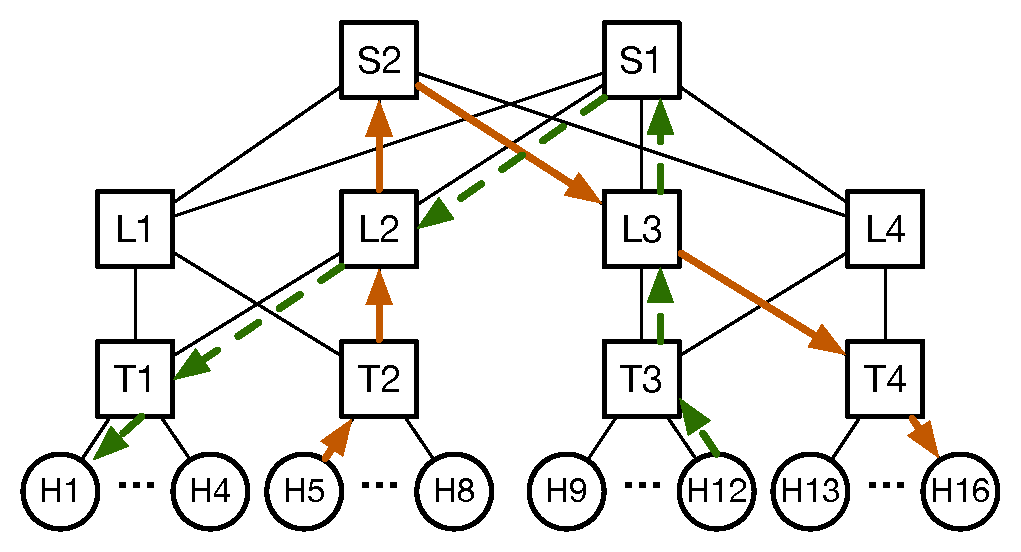
\includegraphics[width=0.45\textwidth] {figs/testbed_topo}
	\caption{Testbed Topology.}\label{fig:testbed_topo}
	\vspace{-0.25in}
\end{figure}

\para{Testbed:} Our testbed consists of a Clos network with 10 switches 16
servers (Figure~\ref{fig:testbed_topo}). Each server is a Dell PowerEdge R730
server with a 40GbE Mellanox ConnectX-3 Pro NIC. Each switch is a Arista
7050 switch with 32 40GbE ports and 16MB packet buffer. The switches
support PFC with at most 8 priority classes.




\subsection{Deadlock prevention}\label{subsec:exp_validation}

\begin{figure}[t]
	%\vspace{-0.1in}
	\centering
	
	\subfloat[short for lof][Without \sysname] {
		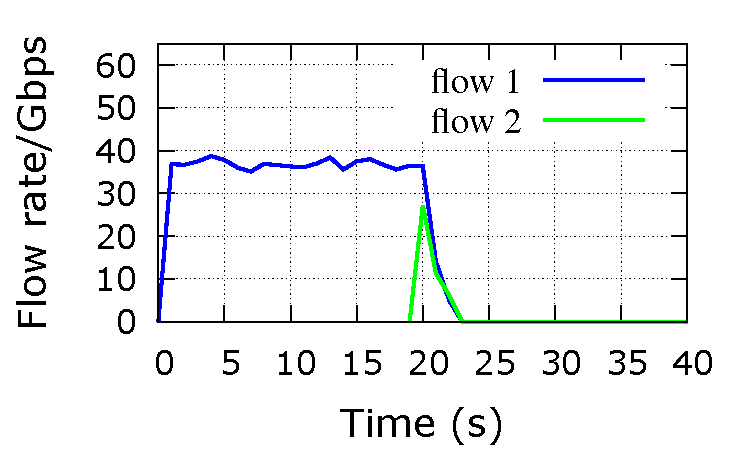
\includegraphics[width=0.25\textwidth] {figs/validation_nonloopcase_flowrate_notagger}
	}
	\subfloat[short for lof][With \sysname]{
		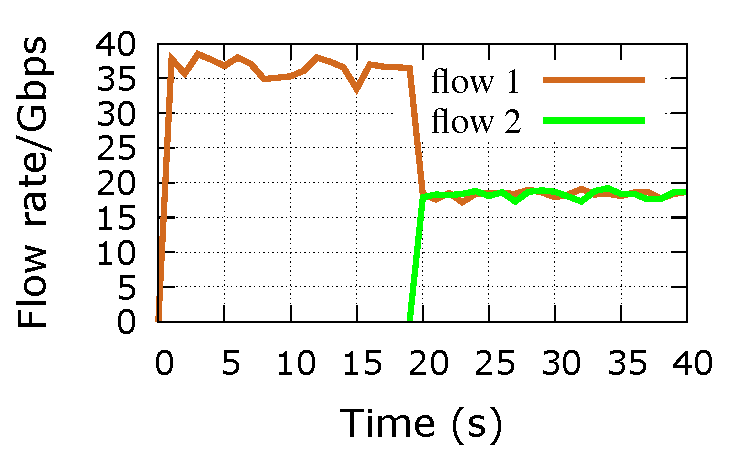
\includegraphics[width=0.25\textwidth] {figs/validation_nonloopcase_flowrate_tagger}
	}
	
	\caption{Clos deadlock due to 1-bounce paths}\label{fig:exp_validation_nonloop}
	\vspace{-0.25in}
\end{figure}

\begin{figure}[t]
	%\vspace{-0.1in}
	\centering
	
	\subfloat[short for lof][Scenario] {
		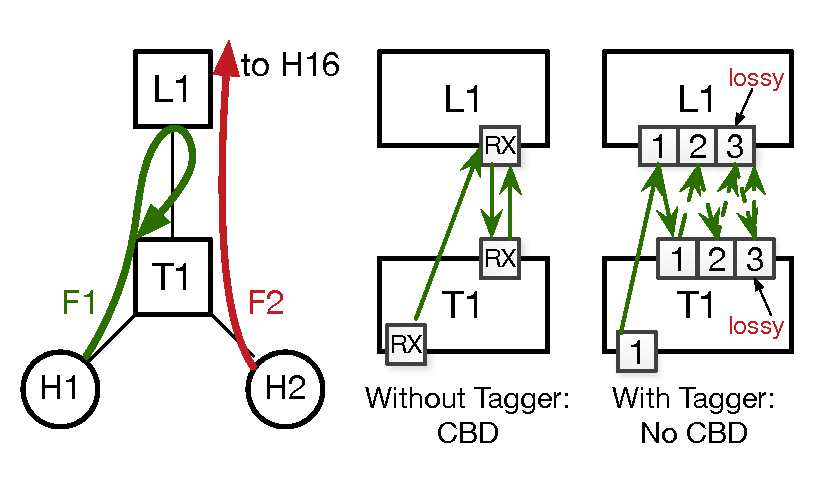
\includegraphics[width=0.4\textwidth] {figs/validation_loopcase_scenario}
	}

\vspace{-0.25in}

	\subfloat[short for lof][Rate of flow 2]{
		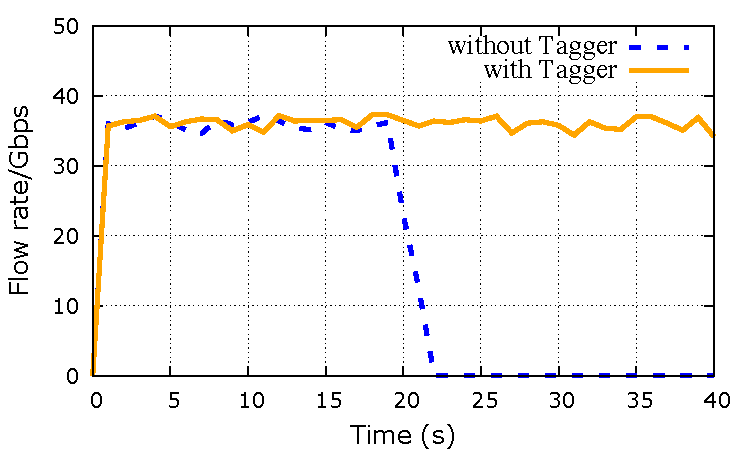
\includegraphics[width=0.4\textwidth] {figs/validation_loopcase_flowrate}
	}
	
	\caption{Deadlock due to routing loop}\label{fig:exp_validation_loop}
	
\end{figure}

\begin{figure}[t]
	%\vspace{-0.1in}
	\centering
	
	\subfloat[short for lof][4-to-1 shuffle with \sysname] {
		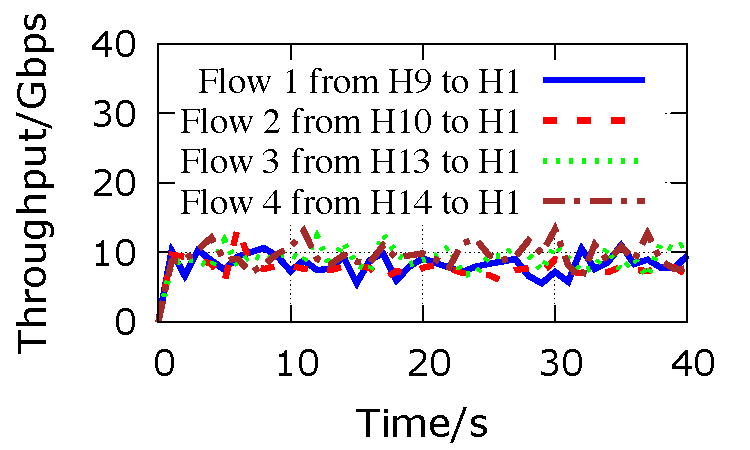
\includegraphics[width=0.25\textwidth] {figs/validation_pp_manytoone_tagger}
	}
	\subfloat[short for lof][4-to-1 shuffle without \sysname]{
		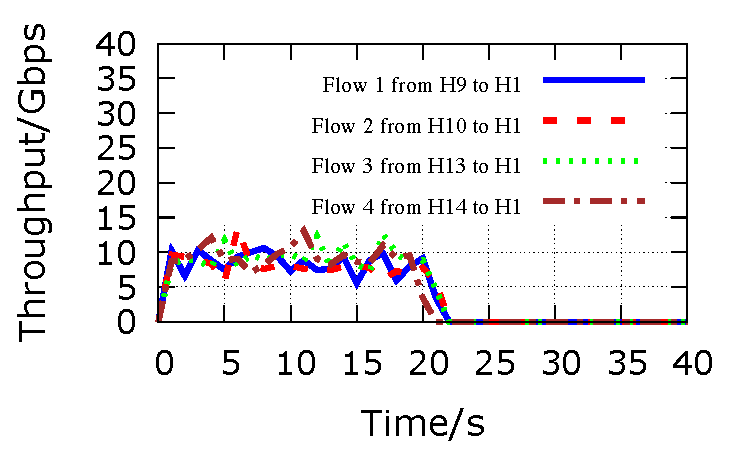
\includegraphics[width=0.25\textwidth] {figs/validation_pp_manytoone_notagger}
	}

	\subfloat[short for lof][1-to-4 shuffle with \sysname] {
	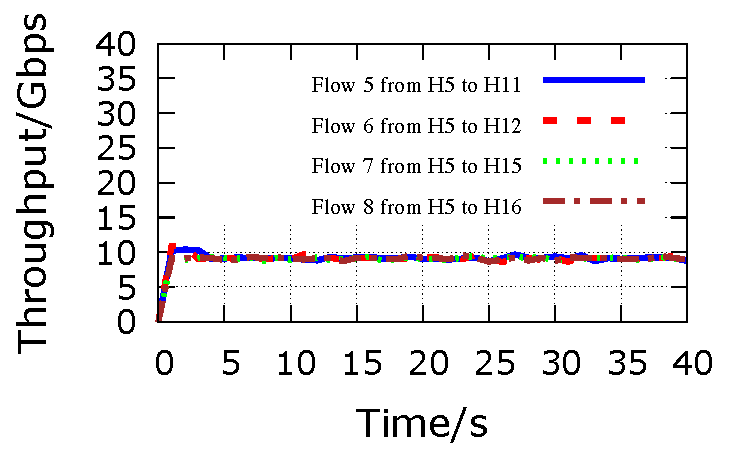
\includegraphics[width=0.25\textwidth] {figs/validation_pp_onetomany_tagger}
}
\subfloat[short for lof][1-to-4 shuffle without \sysname]{
	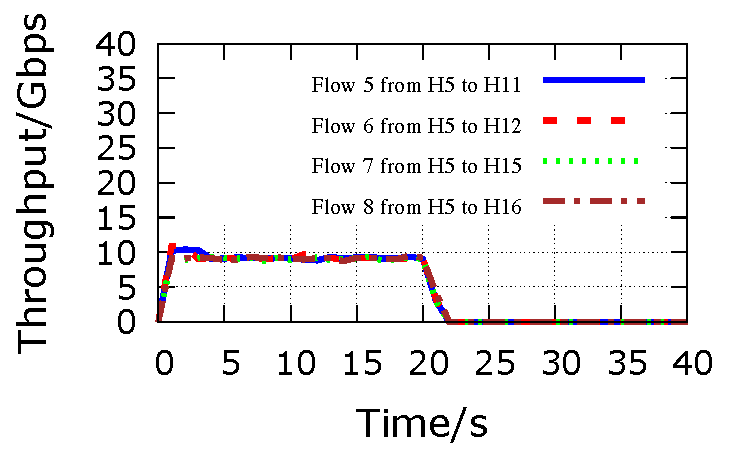
\includegraphics[width=0.25\textwidth] {figs/validation_pp_onetomany_notagger}
}
	
	\caption{PFC PAUSE propagation due to deadlock
	 }\label{fig:exp_validation_propagation}
	
\end{figure}


We have already {\em proved} that \sysname{} prevents deadlock, so the
experiments in this section are primarily illustrative. We have also done
extensive simulations. We omit these for lack of space.

\textbf{Deadlock due to one bounce:} We recreate the scenario shown in
Figure~\ref{fig:clos_1_bounce}, where 1-bounce paths lead to CBD.  In this
experiment, we start the orange flow at time 0, and the green flow at time 20.
Figure~\ref{fig:exp_validation_nonloop} shows the rate of the two flows with and
without \sysname{}.  Without \sysname{}, deadlock occurs and rate of both flows
are reduced to 0. With \sysname{}, and ELR set to include shortest paths and
1-bounce paths, there is no deadlock and flows are not paused.

\textbf{Deadlock due to routing loop:} As shown in
Figure~\ref{fig:exp_validation_loop}(a), we generate 2 flows across different
ToRs, i.e.,  $F_1$ from H1 to H15 and $F_2$ from H2 to H16. At time = 20s, we
install a bad route at L1 to let $F_1$ enter a routing loop between T1 and L1.
The path taken by $F_2$ also traverses link T1-L1.  ELR is set to include the
shortest paths and 1-bounce paths.

In Figure~\ref{fig:exp_validation_loop}(b), we plot the rate of $F_2$ with and
without \sysname{}. As we can see, if \sysname{} is not used, deadlock occurs
and $F_2$ is paused due to propagation of PFC PAUSE. With \sysname{}, there is
no deadlock and $F_2$ is not paused (but rate is affected by the routing loop). Note that
throughput of $F_1$ is zero, as packets are dropped due to TTL expiration.

The key takeaway here is that \sysname{} was able to successfully deal with a
routing loop.

\textbf{PAUSE propagation due to deadlock:} Once deadlock occurs, PFC PAUSE will
propagate and may finally pause all the flow running in the datacenter network.
In this experiment, we run a many-to-one data shuffle from H9, H10, H13 and H14
to H1, and a one-to-many data shuffle from H5 to  H11, H12, H15 and H16
simultaneously.  We then change the routing tables manually so that flow from H9
to H1 and the flow from H5 to H15 take 1-bounce paths. This creates CBD as
discussed earlier.

In Figure~\ref{fig:exp_validation_propagation}, we plot the throughput of all 8
flows with and without \sysname{}. Without \sysname{}, all flows get paused due
to PFC PAUSE propagation and throughput is reduced to zero. With \sysname{},
flows are not affected by link failures.

\subsection{Scalability}
\label{subsec:exp_overhead}

As discussed in \S\ref{sec:challenges}, commodity switches can support only a
limited number of lossless queues.  We have already shown that on a Clos
topology, \sysname{} requires $k+1$ lossless priorities to support paths with
up to $k$ bounces. We now consider other topologies.

\begin{table}[t]
		\footnotesize
	\centering
		\begin{tabular}{|r|r|r|r|r|}
			\hline
				Switches & Ports & Network & Lossless & Max \\
						 &		 & Diameter & Priorities & Rules \\
			\hline
			\hline
			100 & 32 & 6 & 3 &  37 \\
			\hline
			500 & 64 & 6 & 3 & 76 \\
			\hline
			1,000 & 64 & 6 & 3 & 88 \\
			\hline
			2,000 & 64 & 7 & 3 & 98 \\
			\hline
			2,000 (*)  & 64 & 7 & 4 &  135\\
			\hline
			
		\end{tabular} 
		\caption{Rules and priorities required for Jellyfish. Half the ports on
		each switch are connected to servers. ELP is shortest paths for first four entries. ELP for last entry includes additional 20,000 random paths.}
\label{table:jellyfish_shortestpath} \end{table}

Jellyfish topology is an r-regular random graph, characterized by the number of
switches, the number of ports a switch has (n) and the number of ports used to
connect with other switches (r).  In our experiment, we let r = n/2. Remaining
ports are connected to servers. We construct ELP by building destination-rooted
shortest-path spanning trees at all the servers.
Table~\ref{table:jellyfish_shortestpath} shows the results.  

\sysname{} requires only four classes for a network with 2000 switches, even
when 20,000 random routes are used in addition to the shortest paths, and at
most\footnote{Different switches require different number of rules due to the
random nature of the topology.} 135 match-action rules per switch.  Modern
commodity switches can support 1-4K rules, so this is not an issue. 

We also considered smaller (100 switches, 32 ports) Jellyfish topologies with
upto 16-shortest path routing. We need just 2 lossless priorities, and no more
than 47 rules per switch.

BCube~\cite{bcube} is server-centric topology, constructed from servers with $n$
ports, $n^k$ switches with $n$ ports. BCube$(8,3)$ with ELP of $3$ shortest
paths requires 4 lossless priorities, and 41 rules per switch.
F10~\cite{f10} is a fault-tolerant FatTree-like topology.  With three-level
network of 64 port switches, and ELP of all shortest and 1-bounce paths, we need
just 2 lossless priorities and 164 rules per switch.

Generating tagging rules is a one-time activity. Still, runtime of
Algorithm~\ref{alg:greedy} is of possible interest.
Figure.~\ref{fig:algo_runtime} shows the runtime for Jellyfish topologies of
different sizes. Even with 2000 switches, we complete rule generation in about
1.5 hours on a commodity desktop machine.

Thus, we conclude that in terms of number of lossless classes and ACLs,
\sysname{} scales well for modern data center architectures. 

\begin{figure}
	\centering
	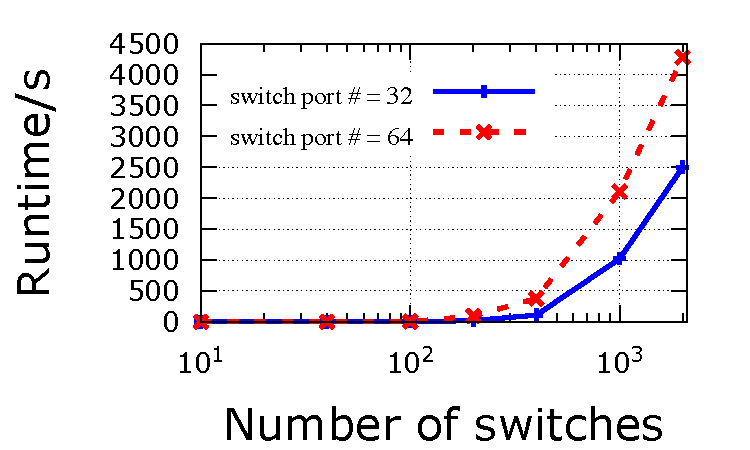
\includegraphics[width=0.45\textwidth] {figs/algo_runtime}
	\caption{Runtime of Algorithm~\ref{alg:greedy} for Jellyfish network of different sizes.}
	\label{fig:algo_runtime}
	\vspace{-0.25in}
\end{figure}

\subsection{Impact on throughout and latency}\label{subsec:exp_performanceoverhead}

\begin{figure}[t]
	\centering
	
	\subfloat[short for lof][Throughput] {
		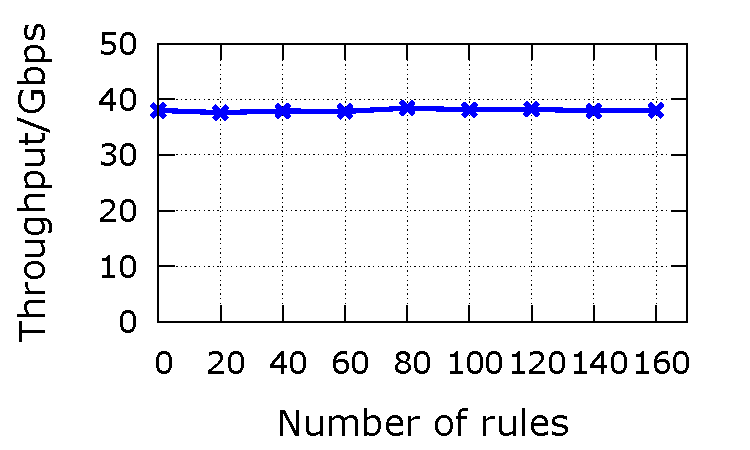
\includegraphics[width=0.25\textwidth] {figs/overhead_avgthrpt}
	}
	\subfloat[short for lof][Latency]{
		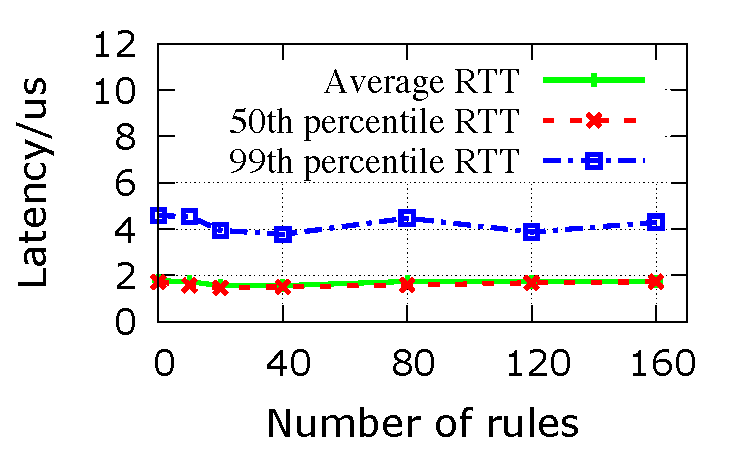
\includegraphics[width=0.25\textwidth] {figs/RDMAlatency_overhead}
	}
	
		\caption{\sysname{} has no impact on throughput and latency}
		\label{fig:perf_penalty}
	\vspace{-0.25in}
\end{figure}

At run time, the only impact of \sysname{} is that the packet has to traverse
the ACL rules. These are installed in TCAM, and hence have no discernible impact
on throughput and latency, as illustrated in Figure~\ref{fig:perf_penalty}.

\textbf{Throughput}: We generate one flow from H1 to H2, and observe its average
throughput over 100 seconds under varying number of \sysname{} rules installed
on T1. Figure~\ref{fig:perf_penalty}(a) shows that the average throughput is not
affected.

\textbf{Latency}: We install different number of \sysname{} rules in T1 and
collect 5000 RTT samples between H1 and H2.  Table~\ref{fig:perf_penalty}(b)
shows that latency is not affected.



%\subsection{Simple demonstration of \sysname{}}\label{subsec:exp_demon}  
%	
%	\begin{figure}[t]
%		%\vspace{-0.1in}
%		\centering
%		
%		\subfloat[short for lof][Experiment scenario.]{
%			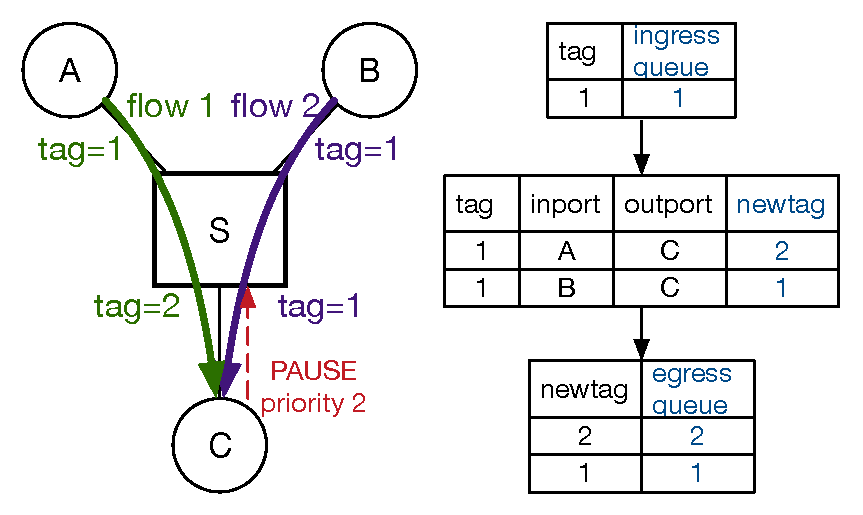
\includegraphics[width=0.25\textwidth] {figs/demon_scenario}
%		}
%		\subfloat[short for lof][Rate of flow 1 and flow 2.]{
%			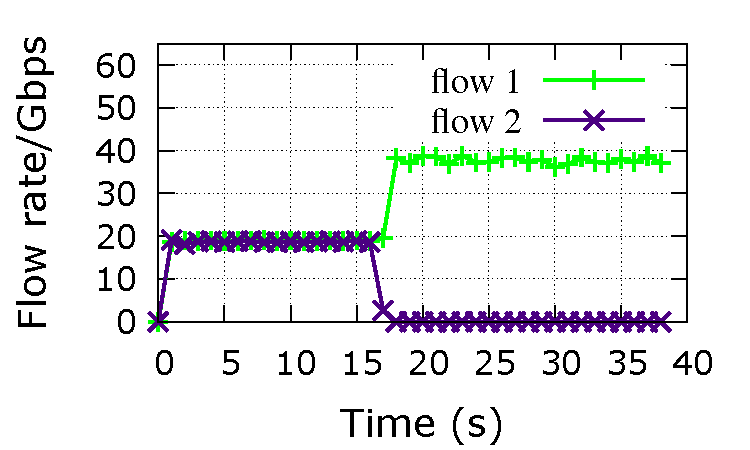
\includegraphics[width=0.25\textwidth] {figs/demon_flowrate}
%		}
%		
%		\caption{The match-action rules in action}\label{fig:tagger_demon}
%	\end{figure}
%	
%	
%A simple experiment shown in
%Figure~\ref{fig:tagger_demon} demonstrates the behavior of the match-action
%rules.  We generate two flows, flow 1 and flow 2, to send packets to C from
%different servers connected to ports A and B. Both servers set the DSCP value in
%outgoing packets to 1. The match-action rules are set to rewrite the tag value
%of packets arriving on port A to 2, and forward them to port C. Tag of packets
%arriving on port B is not changed.
%
%At time = 17s, C sends a stream of forged PFC PAUSE frames on priority 2 to
%switch S. The rate of both flows is plotted in Figure~\ref{fig:tagger_demon}(b)
%(link capacity = 40Gbps). As expected, after priority 2 is paused, rate of
%flow 1 is reduced to 0 while flow 2 gets all the available bandwidth.
%Counters on switch S further confirm that no packets were dropped, and server
%connected to port A was paused as expected.

%%%\vspace{-0.1in}
\section{\sys Applications}\label{sec:application}
%\vspace{-0.1in}
To showcase \sys's utility, we use it for explicit path support in four applications. The key is that, built on \sys, applications can freely choose which path to use without worrying about how to set up the path and the time cost or overhead of setting up the path. In this regard, \sys emerges as an interface for applications to use explicit paths conveniently, but does not make any choice on behalf of them.

%We incorporate \sys into 5 representative applications for routing and demonstrate its utility. For bandwidth-guarantee, we show that \sys's explicit path control makes end-to-end bandwidth provisioning easier to implement. For partition-aggregation application, we show that \sys can express 1-to-$n$ or $n$-to-1 patterns and can be leveraged to give search query high priority for service differentiation. For map-reduce, we show that \sys can express $m$-to-$n$ pattern and the path IDs can used to identify disjoint parallel paths that speedup the many-to-many data shuffle and avoid collision of ECMP.

%\begin{figure}[t]
%\centering
%\subfloat[nooneline, footnotesize][Remaining bandwidth on $P_1$, $P_2$, $P_3$ is 300, 100, 100 Mbps.]
%{\includegraphics[width=0.28\textwidth] {figs/iops-topo.eps}}
%%\vspace{-0.1in}
%\subfloat[nooneline, footnotesize][Average IOPS.] {
%{\scalebox{0.8} {
%\begin{tabular}[b]{|l | c|}
%    \hline
%    & \tabincell{c}{\textbf{Average IOPS}} \\
%    \hline
%    \hline
%    \sys & 15274 \\
%    \hline
%    ECMP & 4547 \\
%    \hline
%\end{tabular}}}}
%
%\subfloat[nooneline, footnotesize][Throughput and completion time of RoX and ECMP.] {
%\includegraphics[width=0.45\textwidth]{figs/iops-throughput.eps}}
%%\vspace{-0.17in}
%\caption{\sys utility case $\#1$: we leverage \sys to make provisioned I/O bandwidth easier to implement.}
%\end{figure}

%\vspace{-0.1in}
\subsection{\sys for provisioned IOPS}\label{subsec:iops}
%\vspace{-0.1in}
%In cloud services, there is an increasing need for bandwidth provisioning. For example, Amazon RDS enforces provisioned I/O bandwidth for instances to ensure that disk resources are always available whenever you need them~\cite{privisionIO}. In this experiment, we show \sys's explicit path control makes end-to-end bandwidth provisioning easy to implement. For the experiment setting, we pick a pod and use background UDP flows to stature the ToR-Agg links and leave the remaining bandwidth on three paths between X-Y as 100Mpbs, 300Mbps, 100Mbps respectively. Suppose now there comes a demand to provision the bandwidth between X-Y at 300Mbps. We then leverage ECMP and \sys to implement it.

\begin{figure}[t]
\centering
%\vspace{-0.1in}
\includegraphics[width=0.5\textwidth,center]{figs/f8.eps}\hspace{-0.2in}
%\vspace{-0.1in}
\caption[Optional caption for list of figures]{\sys utility case $\#1$: we leverage \sys to make necessary bandwidth easier to implement for provisioned IOPS.}
\label{fig:iops}
\vspace{-0.2in}
\end{figure}

In cloud services, there is an increasing need for provisioned IOPS. For example, Amazon EBS enforces provisioned IOPS for instances to ensure that disk resources can be accessed with high and consistent I/O performance whenever you need them~\cite{privisionIO-EBS}. To enforce such provisioned IOPS, it should first provide necessary bandwidth for the instances~\cite{io-characteristics}. In this experiment, we show \sys can be easily leveraged to use the explicit path with necessary bandwidth.

As shown in Fig.~\ref{fig:iops}(a), we use background UDP flows to stature the ToR-Agg links and leave the remaining bandwidth on 3 paths ($P_1, P_2$ and $P_3$) between X-Y as 300Mpbs, 100Mbps, and 100Mbps respectively. Suppose there is a request for provisioned IOPS that requires 500Mbps necessary bandwidth (The provisioned IOPS is about 15000 and the chunk size is 4KB.). We now leverage \sys and ECMP to write 15GB data ($\approx$4 million chunks) through 30 flows from X to Y, and measure the achieved IOPS respectively. The storage we used for the experiment is Kingston V+200 120G SSD, and the I/O operations on the storage are sequential read and sequential write.

\begin{figure}[t]
\centering
\vspace{-0.15in}
\subfloat[short for lof][Path $P_1$: T1~$\rightarrow$A1~$\rightarrow$T3; $P_2$: T1~$\rightarrow$A2~$\rightarrow$T3; $P_3$: T1~$\rightarrow$A3~$\rightarrow$T3] {
    \includegraphics[width=0.40\textwidth] {figs/updt-topo.eps}
    \label{fig:network-update_a}
}
\vspace{-0.15in}

\subfloat[short for lof][Time $t_1$: move $f_3$ from $P_2$ to $P_3$;~ $t_2$: move $f_1$ from $P_1$ to $P_2$;~$t_3$: move $f_1$ from $P_2$ to $P_1$;~ $t_4$: move $f_3$ from $P_3$ to $P_2$.]{
    \includegraphics[width=0.40\textwidth] {figs/updt-mat-new.eps}
    \label{fig:network-update_b}
}
\vspace{-0.1in}
\caption[Optional caption for list of figures]{\sys utility case \#2: we leverage XPath to assist zUpdate~\cite{zupdate} to accomplish DCN update with zero loss.}
\label{fig:network-update}
\vspace{-0.2in}
\end{figure}

From Fig.~\ref{fig:iops}(c), it can be seen that using ECMP we cannot provide the necessary bandwidth between X-Y for the provisioned IOPS although the physical capacity is there. Thus, the actual achieved IOPS is only 4547, and the write under ECMP takes much longer time than that under \sys as shown in Fig.~\ref{fig:iops}(c). This is because ECMP performs random hashing and cannot specify the explicit path to use, hence it cannot accurately make use of the remaining bandwidth on each of the multiple paths for end-to-end bandwidth provisioning. In contrast, \sys can be easily leveraged to provide the required bandwidth due to its explicit path control. With \sys, we explicitly control how to use the three paths and accurately provide 500Mbps necessary bandwidth, achieving 15274 IOPS.


%\vspace{-0.05in}
\subsection{\sys for network updating}\label{subsec:update}
\vspace{-0.05in}
In production data centers, DCN update occurs frequently~\cite{zupdate}. It can be triggered by the operators, applications and various networking failures. zUpdate~\cite{zupdate} is an application that aims to perform congestion-free network-wide traffic migration during DCN updates with zero loss and zero human effort. In order to achieve its goal, zUpdate requires explicit routing path control over the underlying DCNs. In this experiment, we show how \sys assists zUpdate to accomplish DCN update and use a switch firmware upgrade example to show how traffic migration is conducted with \sys.

In Fig.~\ref{fig:network-update}(a), initially we assume 4 flows ($f_1, f_2, f_3$ and $f_4$) on three paths ($P_1, P_2$ and $P_3$). Then we move $f_1$ away from switch $A_1$ to do a firmware upgrade for switch $A_1$. However, neither $P_2$ nor $P_3$ has enough spare bandwidth to accommodate $f_1$ at this point of time. Therefore we need to move $f_3$ from $P_2$ to $P_3$ in advance. Finally, after the completion of firmware upgrade, we move all the flows back to original paths. We leverage \sys to implement the whole movement.

\begin{figure}[t]
\centering
%\vspace{-0.2in}
\includegraphics[width=0.45\textwidth]{figs/be.eps}
%\vspace{-0.15in}
\caption{\sys utility case $\#3$: we leverage \sys to accurately enforce VDC with bandwidth guarantees.}
\label{fig:bandwidth_enforcement}
\vspace{-0.2in}
\end{figure}

In Fig.~\ref{fig:network-update}(b), we depict the link utilization dynamics. At time $t_1$, when $f_3$ is moved from $P_2$ to $P_3$, the link utilization of $P_2$ drops from 0.6 to 0.4 and the link utilization of $P_3$ increases from 0.7 to 0.9. At time $t_2$, when $f_1$ is moved from $P_1$ to $P_2$, the link utilization of $P_1$ drops from 0.5 to 0 and the link utilization of $P_2$ increases from 0.4 to 0.9. The figure also shows the changes of the link utilization at time $t_3$ and $t_4$ when moving $f_3$ back to $P_2$ and $f_1$ back to $P_1$. It is easy to see that with the help of \sys, $P_1, P_2$ and $P_3$ see no congestion and DCN update proceeds smoothly without loss.

%Compared to OpenFlow, since \sys is capable to pre-install large number of paths into IP tables, zUpdate doesn't need to change the flow and group tables on switches in every step of the traffic migration. For most of the cases, \sys only needs to notify the senders to transfer a part of flows to some other paths.

%\vspace{-0.1in}
\subsection{Virtual network enforcement with \sys}\label{subsec:vne}
%\vspace{-0.05in}
%
%\begin{figure*}[ht]
%\centering
%\subfloat[short for lof][The Fattree(6) testbed with 54 servers we implemented. Each ToR switch connects 3 servers (not drawn).] {
%    \includegraphics[width=0.32\textwidth] {figs/testbed-topo}
%    \label{fig:fattree}
%}
%\vspace{-0.17in}\hfill
%\subfloat[short for lof][\sys utility case $\#4$: we leverage \sys to express partition-aggregation traffic pattern ($1$-to-$n$, $n$-to-$1$) and enforce service differentiation.] {
%    \includegraphics[width=0.33\textwidth] {figs/pa.eps}
%    \label{fig:partition_aggregation_query}
%}\hfill
%\subfloat[short for lof][\sys utility case $\#5$: we leverage \sys to select non-conflict paths to speed up many-to-many data shuffle.]{
%    \includegraphics[width=0.3\textwidth] {figs/shuffle}
%    \label{fig:shuffle}
%}
%\caption[Optional caption for list of figures]{}
%\label{fig:network-update}
%\vspace{-0.2in}
%\end{figure*}


In cloud computing, virtual data center (VDC) abstraction with bandwidth guarantees is an appealing model due to its performance predictability in shared environments~\cite{secondnet,oktopus,proteus2012}. In this experiment, we show \sys can be applied to enforce virtual networks with bandwidth guarantees. We assume a simple SecondNet-based VDC model with 4 virtual links, and the bandwidth requirements on them are 50Mbps, 200Mbps, 250Mbps and 400Mbps respectively as shown in Fig.~\ref{fig:bandwidth_enforcement}(a). We then leverage \sys's explicit path control to embed this VDC into the physical topology.

In Fig.~\ref{fig:bandwidth_enforcement}(b), we show that \sys can easily be employed to use the explicit paths in the physical topology with enough bandwidth to embed the virtual links. In Fig.~\ref{fig:bandwidth_enforcement}(c), we measure the actual bandwidth for each virtual link and show that the desired bandwidth is accurately enforced. However, we found that ECMP cannot be used to accurately enable this because ECMP cannot control paths explicitly.

%\vspace{-0.2in}
%\subsection{\sys support for partition-aggregation query}\label{subsec:partition}
%\vspace{-0.1in}
%In web applications, the partition-aggregation paradigm is a foundation for many online services such as search query. They usually generate one-to-many and many-to-one communication patterns and has very demanding latency requirements. Using \sys, we can explicitly express such 1-to-$n$ and $n$-to-1 patterns using ($n$+1) path IDs, one ID for $n$-to-1 and $n$ IDs for 1-to-$n$. These IDs form a group that can be leveraged for optimizations such as service differentiation.
%
%In this experiment, we selected 9 servers in a pod to emulate a 1-to-8 (8-to-1) query-and-response, and we used 9 IDs to express such group communication patterns. We saturate the network with background traffic, and then leverage such 9 IDs to set priority to such query-and-response traffic.
%
%\begin{figure}[t]
%\vspace{-0.1in}
%\centering
%\includegraphics[width=0.45\textwidth]{figs/pa.eps}
%\vspace{-0.1in}
%\caption{\sys utility case $\#4$: we leverage \sys to express partition-aggregation traffic pattern ($1$-to-$n$, $n$-to-$1$) and enforce service differentiation.}
%\label{fig:partition_aggregation_query}
%\vspace{-0.25in}
%\end{figure}
%
%
%
%In Fig.~\ref{fig:partition_aggregation_query}, we found that when the group of path IDs are referenced for priority, the query flows see persistently low RTTs of less than 200$\mu$s irrespective of the background traffic. However, if we do not set up a priority for these IDs, the RTT increases to the millisecond level as the background load increases. This experiment showcases \sys's utility in service differentiation for partition-aggregation queries.

%\vspace{-0.1in}
\subsection{Map-reduce data shuffle with \sys}\label{mapreduce}
%\vspace{-0.1in}
In Map-reduce applications, many-to-many data shuffle between the map and reduce stages can be time-consuming. For example, Hadoop traces from Facebook show that, on average, transferring data between successive stages accounts for $33\%$ of the running times of jobs~\cite{orchestra}. Using \sys, we can explicitly express non-conflict parallel paths to speed up such many-to-many data shuffle. Usually, for a $m$-to-$n$ data shuffle, we can use ($m$+$n$) path IDs to express the communication patterns. The shuffle patterns can be predicted using existing techniques~\cite{hadoopwatch}.

\begin{figure}[t]
%\vspace{-0.1in}
\centering
\includegraphics[width=0.5\textwidth]{figs/shuffle}
\vspace{-0.2in}
\caption{\sys utility case $\#4$: we leverage \sys to select non-conflict paths to speed up many-to-many data shuffle.}
\label{fig:shuffle}
\vspace{-0.2in}
\end{figure}

In this experiment, we selected 18 servers in two pods of the Fattree to emulate a 9-to-9 data shuffle by letting 9 servers in one pod send data to 9 servers in the other pod. We varied the data volume from 40G to over 400G. We compared \sys with ECMP.

In Fig.~\ref{fig:shuffle}, it can be seen that by using \sys for data shuffle, we can perform considerably better than randomized ECMP hash-based routing. More specifically, it reduces the shuffle time by over 3$\times$ for most of the experiments. The reason is that \sys's explicit path IDs can be easily leveraged to arrange non-interfering paths for shuffling, thus the network bisection bandwidth is fully utilized for speedup.


%We further note that \sys can simply use 3 path IDs to express such many-to-many communication patterns, which makes the non-conflict parallel path arrangement fairly easy to implement.



%%%\vspace{-0.1in}
\section{Related Work}\label{sec:related}

\para{Deadlock-free routing.} Many Deadlock-free routing designs have been
proposed. See
\cite{dally,duato93,dally93,sancho2004,flich2012survey,lash,wu2003fault,glass,duato2001,domke2011,puente1999,dfedst16}
for representative schemes. Generally, these designs prevent deadlock by
imposing restrictions on the routing paths, and can be classified into two
categories.

The first category is {\em deterministic routing based approach}, in which the
routing path is not affected by the traffic status, and there is no CBD.  These
routing algorithms are not compatible with existing routing protocols including
OSFP and BGP. Worse, they cannot be implemented in current commodity switching
ASICs.

TCP-Bolt~\cite{tcpbolt} and DF-EDST~\cite{dfedst16} are two recently
proposed deadlock-free routing designs. They both build edge-disjoint
spanning trees (EDSTs), with DF-EDST~\cite{dfedst16} further builds a
deadlock-free tree transition acyclic graph such that the transition
among some EDSTs can be allowed. However, existing L3 routing protocols
do not guarantee that packets will follow the pre-assign EDSTs, especially
upon link failures. Current switching ASIC cannot detect and handle all 
the potential EDST transition properly.

%support EDST.
%Furthermore, these designs need many EDSTs and
%every EDST needs to occupy a lossless queue. 
%Current switching ASIC,
%however, can only support 2-3 lossless queues.

The second category is {\em adaptive routing based approach.} The key idea is to
pre-install  ``escape'' paths at every switch to cover all possible
destinations. The switches can reroute packets to the ``escape'' paths in the
presence of congestion so that deadlock can be avoided.  As far as we know, no
commodity switching ASIC supports dynamic reroute based on traffic / queue
status.

\para{Intel Omni-Path.} Intel Omni-Path architecture \cite{omnipath} uses the
concept of Service Channels (SC) for routing deadlock avoidance.  Unlike
\sysname{}, Ommi-path uses a centralized fabric manager to manage the
network~\cite{omnipath}, including setting up SCs. This is not feasible at
data center scale.

%% Technical details of Omni-Path are not currently available, Tagger differs
%% from Omni-Path in two significant ways. First, Omni-path needs a fabric
%% manager to dynamically setup SC whereas the tag match-action rules are
%% pre-computed and statically configured. Second, Tagger enforces that
%% the tag of a packet increases monotonically whereas Omni-Path does not
%% enforce order for SC.

\para{Buffer management for deadlock prevention.} It has been shown that by
increasing the packet priority hop-by-hop, and putting packets of different
priority into different buffers, deadlock can be avoided
\cite{firstpaper,survey,datanetworks,karol2003prevention}. These designs,
however, need a large number lossless queues (which is the diameter of the
network). In \cite{dag}, the author tried to reduce the number of lossless
queues to only two. The design does not guarantee losslessness. Furthermore,
some switches need much larger buffer space than the others. 

\para{Deadlock recovery.} Deadlock recovery schemes
\cite{isca95,shpiner2016unlocking,venkatramani1996,martinez1997,Lopez1998}
detect deadlocks once they occur, and then try to break them by rerouting
packets.  These approaches have two issues: (1) They cannot guarantee that
deadlock will not happen again (if they can, there will be no need for deadlock
recovery). (2) They cannot be deployed using existing switch hardware.

%% need to add new deadlock detection algorithms and deadlock
%% breaking protocols into the switches.

%\para{Circuit switching-based approaches.} Those solutions from HPC and InfiniBand
%work by preemption. This does not work in Ethernet and in practice.

\para{Deadlock-free routing reconfiguration}:
Several deadlock-free routing reconfiguration schemes
\cite{automatic,lysne2005,doublescheme,gara2005} have been proposed for
ensuring deadlock-free during routing reconfiguration. \sysname{} can
be used to help any routing protocol to be deadlock-free, as
\sysname{} is decoupled from the routing protocols.

%The basic idea is to divide the reconfiguration process into multiple
%stages, and guarantee deadlock-free routing within each stage. We
%believe
%\sysname{} can be easily modified to guarantee deadlock-free of each
%reconfiguration stage.

\para{Summary.} \sysname{} is different from prior work because it works with
any routing protocol, and with existing hardware. We further have shown that
\sysname{} needs only small number of lossless queues.

%We believe that deciding the priority of packets along the path is
%better than changing routing configurations.

%Deadlock-free routing \cite{dally,duato93,dally93,sancho2004,flich2012survey,lash,wu2003fault,glass,duato2001,domke2011,puente1999} can be achieved by splitting the physical links into virtual channels and virtual channels are arranged in a way so as to avoid circular buffer dependency. In all those designs, the routing is decided by the virtual channels. Hence they cannot work with existing routing protocols for the data center networks which was designed for the lossy networks.
%can be achieved by splitting the physical links into virtual channels and virtual channels are arranged in a way so as to avoid circular buffer dependency. In all those designs, the routing is decided by the virtual channels. Hence they cannot work with existing routing protocols for the data center networks which was designed for the lossy networks.

%%TCP-Bolt~\cite{tcpbolt} uses multiple edge-disjoint spanning trees (EDSTs) and puts every EDST into a separate VLAN and lossless queue to achieve deadlock-free. In addition to the above drawbacks, to achieve good performance, TCP-Bolt may need a large number of lossless queues (which cannot be provided in current commodity switches). Furthermore, TCP-Bolt needs to run layer-2 VLAN, whereas all large-scale data center networks run layer-3.
%
%%DF-EDST~\cite{dfedst16} introduces a set of edge-disjoint spanning trees and a tree transition graph to provide deadlock free routing for arbitrary data center network topologies. DF-EDST, however, cannot work with existing routing protocols as it needs to follow the EDSTs. Furthermore, The EDST selection and transition cannot be readily implemented in current Ethernet switches.

%\secspacelarge
\section{Conclusion}
\secspace

In this paper, we studied the problem of deadlock in datacenter networks.  We
showed that CBD is a {\em necessary} by not {\em
sufficient} condition for deadlock formation. We are unable to fully characterize
the sufficient conditions, but using insights gained from a few examples, we
discussed potential deadlock mitigation mechanisms including TTL-based schemes,
rate limiting and reducing PFC propagation.


%\input{sections/acknowledgement.tex}
%%\begin{small}
%\vspace{-0.05in}
%\bibliographystyle{IEEEtran}
%\bibliography{reference}
%\end{small}
%\begin{appendices}
\section{PFC headroom calculation}\label{APPHEADROOM}

The PFC headroom needed per port per lossless queue can be calculated by
		considering the time interval needed for a receiver to pause its
		upstream sender. The time interval is composed of the following 6
		periods for the lossless class $p$:

	
\noindent\textbf{The time to send a PAUSE frame $t_1$}.  Once a pause frame is
		generated, it may be blocked by a packet that has just started
		transmision. Since Ethernet is non-preemptive, in the worst-cast,
		$t_1 = \frac{ L_{mtu} + L_{pfc}}{B}$, where $L_{mtu}$ is the MTU size,
		and $L_{pfc}$ is the size of a PFC pause frame, and $B$ is the link
		rate.


\noindent\textbf{The PAUSE frame propagation time $t_2$}. This depends on 
		the cable length between the sender and receiver.

\noindent\textbf{The PAUSE frame receiving time at the sender $t3$}.
		$t_3=\frac{L_{pfc}}{B}$.

\noindent\textbf{The PFC response time $t_4$}. This is the amount of time needed
		for the sender to process the pause frame.

\noindent\textbf{The time for the sender to stop transmitting $t_5$}. Again,
		because Ethernet is non-preemptive, sender must to finish 
		transmitting the packet that may have already started. Hence, in the
		worst case, $t_5 =
		\frac{L^{p}_{mtu}}{B}$.

\noindent\textbf{The time for the pipe to be drained $t_6$}. We know $t_6 =
		t_2$.


At a first glance, the headroom size should be $B\times\sum t_i$. But there are
some additional details. The switching ASICs typically divide a packet
into small cells of equal size for internal packet storage and
processing. The cell size ($C$) is typically larger than the smallest
Ethernet packet size (64 bytes). For one 64-byte packet, one cell is
allocated. So in the worst-case, the needed headroom size is:
\begin{eqnarray} \label{eqn:pfcheadroom} S_{hdr} & = &
C\lceil\frac{(t_1+t_2+t_3+t_4 + t_6)B}{64}\rceil + C\lceil \frac{t_5
B}{64}\rceil \nonumber \end{eqnarray}

For a typical 40GbE RoCEv2 setup, we have $L_{mtu}=1500$ bytes, $L_{pfc}=64$
bytes, $t_2=t_6=1us$ (for about 200 meters cable length), $t_4=2.75us$,
$L^{p}_{mtu}=1100$ bytes, $C=208$ bytes.  For a commodity switch with 32
full duplex 40GbE ports, the total headroom size needed is 2.76MB for
supporting one lossless queue.  

\section{Optimal tagging scheme for Clos network}
\label{sec:clos_optimal}

Algorithm~\ref{alg:clos} produces optimal tagging for Clos networks. Note
similarity to Algorithm~\ref{alg:ttl}, except for the last step, which is
specific to Clos networks.

\begin{algorithm}
	\small
    \KwIn{Clos topology and lossless routes $R$}
	\KwOut{A tagged graph $G(V, E)$}
	$V \gets Set()$\;
	$E \gets Set()$\; 
	\For{each path $r$ in $R$} {
		$tag \gets 0$\;
		\For{each hop $h$ in $r$} {
			$V \gets V \cup \{(h, tag)\}$\;
			$E \gets E \cup \{lastHop\rightarrow(h, tag)\}$\;
			\If{$h$ is going down \&\& nextHop is going up} {
				$tag \gets tag+1$\;
			}
		}
	}
	\Return{$G(V, E)$}\;
    \caption{The optimal tagging system for Clos topology.}
	\label{alg:clos}
\end{algorithm}
\end{appendices}


\end{document}
